\chapter{ Specificari Back-end}
\label{chap:ch5}

\par Pe partea de back end sunt prezente doua servere, unul scris in JavaScript cu ajutorul framework-ului Node js care serveste partea de front-end cu toate datele de care are nevoie si un server scris in Python cu ajutorul framework-ului Flask cu ajutorul caruia aflu filme recomandate pentru un film sau o lista  de filme.

\section{Baza de date}
\label{sec:ch5sec1}

\begin{figure}[htbp]
\centerline{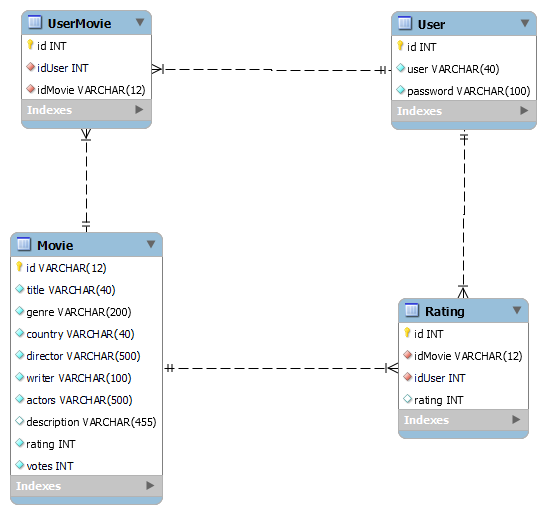
\includegraphics[width=10cm, height=10cm]{figures/diagrama db.png}}
\caption{Diagrama baza de date.}
\label{fig}
\end{figure}

\par Un lucru foarte important in dezvoltarea aplicatiei a fost alegerea bazei de date, am optat pentru pentru MySql versiunea 8.0. In tabelul de User voi salva datele de inregisrare a unui utilizator , in tabelul  Movie sunt prezente datele care descriu un film prin colloanele:title,genre,country,directors,writers,actors,description,votes si rating, in tabelul Rating salvez datele unui rating dat de un user pe laga valoare ratingului salvez si id-urile de la film si user pentru a stii cine da rating si la ce film totodata pe partea de back-end fac si o actualizare a rating ului si numarului de voturi din tabelul Movie asta pentru o a face aplicatia sa se miste mai rapid, iar in tabelul UserMovie salvez id ul de la un user si id ul de la un film reprezentand un film pe care utilizatorul l-a vizualizat.

\section{Server Node Js}
\label{sec:ch5sec1}

\par Serverul de Node Js il folosesc pentru a face inregistrare, login, returanrea tuturor filmelor care contin un numit sub titlu, adaugarea unui film la lista utilizatorului, returnarea a tuturor filmelor unui utilizator si adaugarea de rating a unui film. Cu ajutorul pachetului Express stabilesc rutele si pornesc serverul. Cand se face un request pe o ruta, se apeleaza functia asignata din Service, care are rol de a modela datele in functie de cum avem nevoie. Pentru a comunica cu baza de date ne folosim de Repository, acesta face legatura cu baza de date.

		\begin{figure}[htbp]
			\centerline{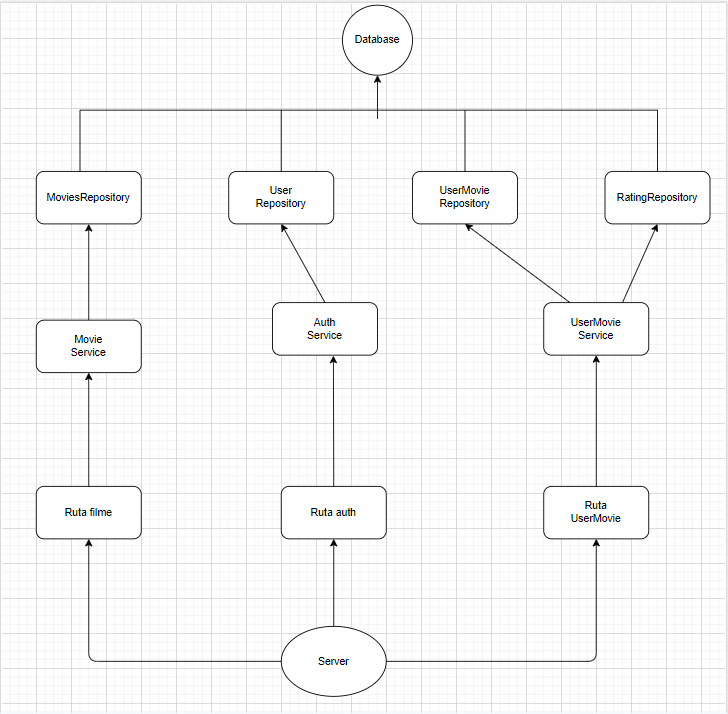
\includegraphics[width=13cm, height=10cm]{figures/diagrama clase node js.png}}
			\caption{Arhitectura server Node Js .}
			\label{fig}
		\end{figure}

\subsection{Inregistrare}
\par Procesul de inregistrare este unul simplu, pasii fiind urmatorii:
\begin{enumerate}
  	\item Se trimit datele catre server
  	\item Se valideaza datele primite 
 	\item Daca datele sunt valide se verifica daca numele utilizatorului se afla in baza de date deoarece numele trebuie sa fie unic pentru fiecare utiliztor
	\item Daca totul este bine pana la acest pas se face has la parola pentru o mai buna securitate
		\begin{figure}[htbp]
			\centerline{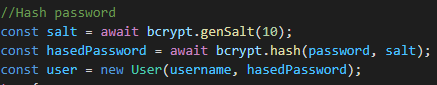
\includegraphics[width=15cm, height=4cm]{figures/hasparola.png}}
			\caption{Has la parola.}
			\label{fig}
		\end{figure}
	\item Următorul pas este de a apela functția din repositoy care adaugă un user in baza de date.
		\begin{figure}[htbp]
			\centerline{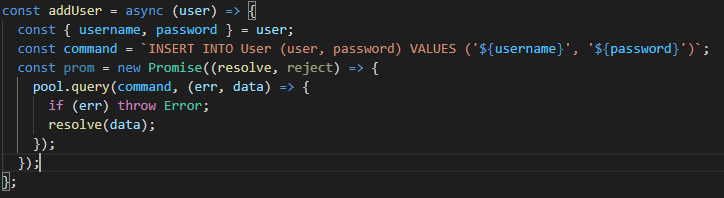
\includegraphics[width=19cm, height=6cm]{figures/adaugare user.png}}
			\caption{Adaugare user in baza de date.}
			\label{fig}
		\end{figure}	
	\item Dacă adăugarea s-a efectuat cu succes se returneaza un messaj de succes altfel se returnează un mesajul de eroare.
\end{enumerate}

\subsection{Autentificare}
\par Pașii pentru procesul de autentificare sunt următorii
\begin{enumerate}
  	\item Se trimit datele catre server
  	\item Se valideaza datele primite
  	\item Se verifica daca username-ul se afla in baza de date 
		\begin{figure}[htbp]
			\centerline{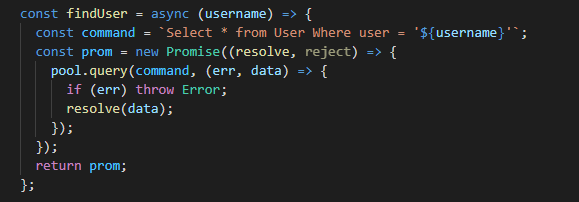
\includegraphics[width=19cm, height=6cm]{figures/cautare user.png}}
			\caption{Cautare dupa username in baza de date}
			\label{fig}
		\end{figure}	
	\item Daca se găsește user-ul in baza de date se verifică parola trimisă in requst cu cea din baza de date apoi se trimite raspunsul in functie de potrivirea celor doua parole, daca rapunsul este valid se va trimite id-ul user-ului care va reprezenta token-ul pentru front-end, daca  parolele nu corespund se va trimite status 400 si un mesaj de eroare.
		\begin{figure}[htbp]
			\centerline{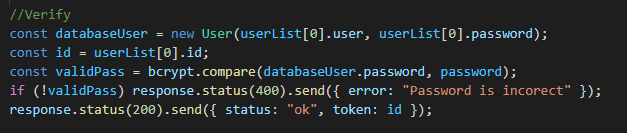
\includegraphics[width=19cm, height=6cm]{figures/verificare login.png}}
			\caption{Verificare parola si trimitere raspuns}
			\label{fig}
		\end{figure}	
\end{enumerate}


\subsection{Lista filmelor care contin un subtitlu}
\par Pașii pentru returnarea listii sunt:
\begin{enumerate}
  	\item Dupa se se apeleaza ruta specifica se ia din body titlul
  	\item Se apeleaza functioa din repository care returneaza lista
  	\item In repository se iau toate filmele din baza de date apoi se parcurg pentru a pastra doar filmele care contin subtitlul dat.
		\begin{figure}[htbp]
			\centerline{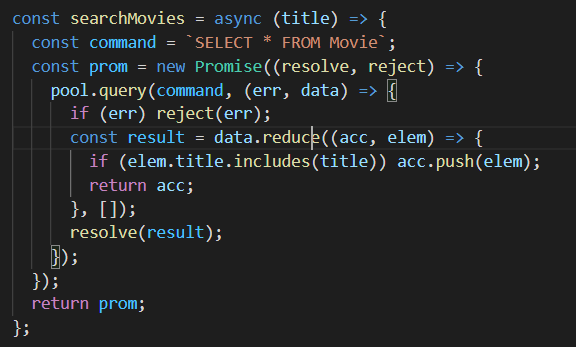
\includegraphics[width=19cm, height=6cm]{figures/cautarea filme.png}}
			\caption{Functia din repository care cauta filmele}
			\label{fig}
		\end{figure}	
			
\end{enumerate}

